\chapter{ Introducción Específica } % Main chapter title
%----------------------------------------------------------------------------------------
%	INTRODUCCION
%----------------------------------------------------------------------------------------
Aquí se abordan con mas detalle el proceso de fabricación, los parámetros críticos y las fallas que pueden derivarse. Luego se exponen los criterios de diseño del prototipo a partir de los casos de uso del mismo, modos de funcionamiento. Finalmente se detalla la lista de requerimientos completos, a saber: funcionales y no funcionales, de interfaz, de diseño y futuros.

\section{ Galvanizado de circuitos impresos }

El proceso de galvanizado consiste en adherir a un objeto metálico una delgada capa de otro metal, de unos pocos micrones de espesor. Este material le otorga mejores propiedades al objeto como ser conductividad eléctrica, mayor resistencia mecánica o resistencia a la corrosión. 

Los métodos para lograrlos pueden ser diversos. Entre los mas comunes están el baño químico y por electrólisis. El método químico es utilizado generalmente en estructuras con superficies homogéneas y consiste en sumergir el producto dentro de un baño con el metal galvanizante en forma de solución química o bien a alta temperatura, incluyendo algunas etapas de pre- acondicionado. La figura \ref{fig:galvanizado_quimico} es un diagrama simplificado de método químico.
El método electrolítico insume un gran consumo de energía eléctrica y mas etapas de pre-tratamiento de la superficie, pero tiene la ventaja de ser mas controlable el grosor del galvanizado, se suele hacer a temperatura ambiente y es mas versátil para aplicar sobre superficies no metálicas con un pre acondicionado previo. En la figura \ref{fig:galvanizado_electrolitico} se  un proceso electrolítico donde básicamente el objeto recibe distintos pre-tratamientos para preparar la superficie antes y después del efecto electrolítico. 

\hspace{1px}
\begin{figure}[h]
	\centering
	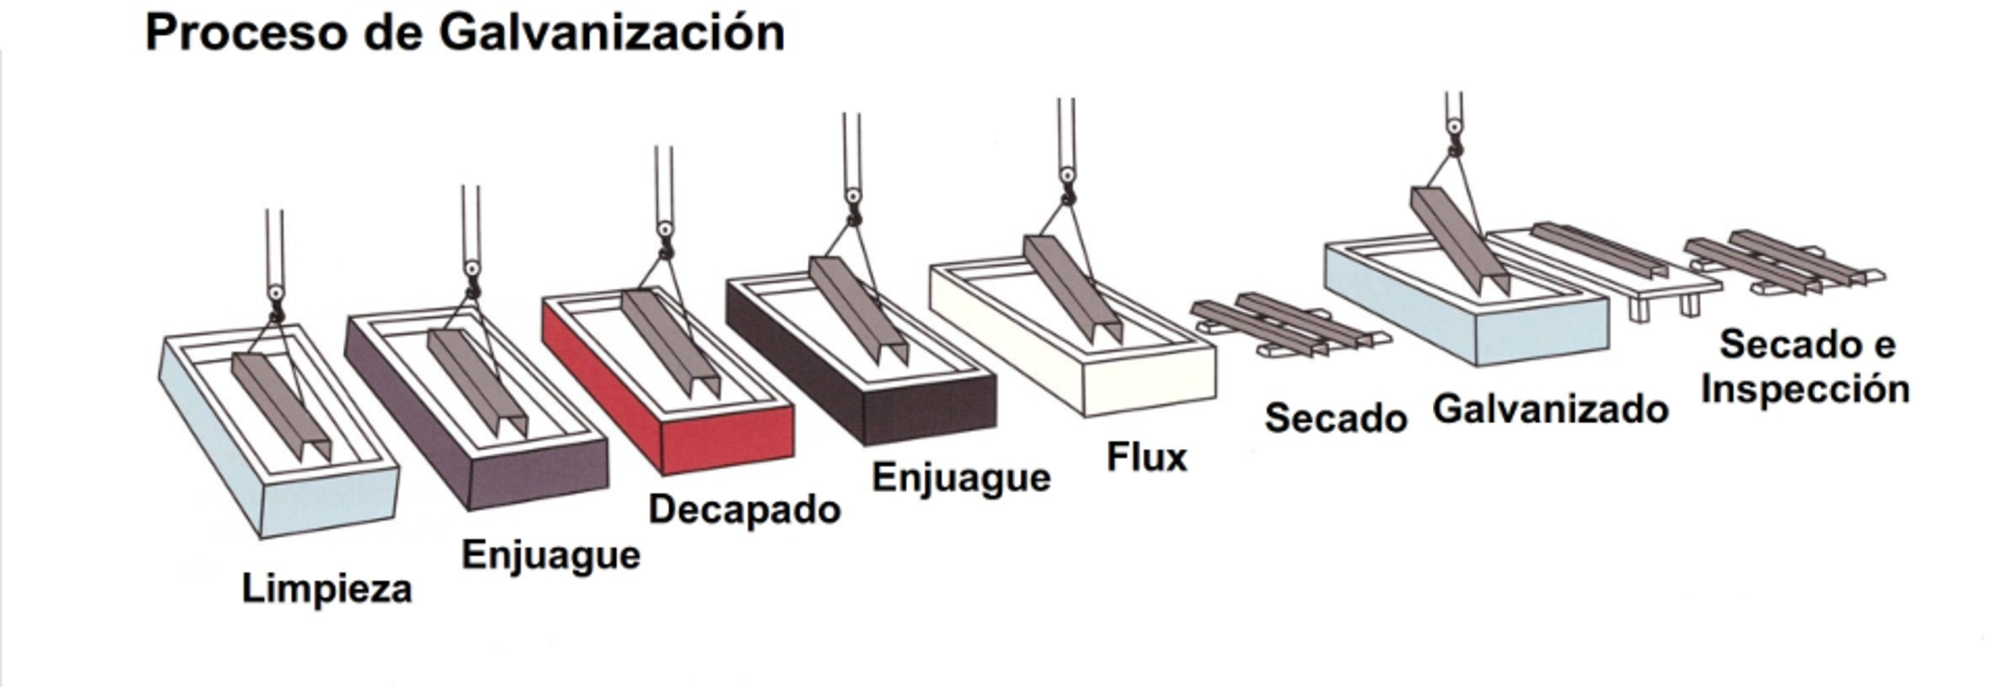
\includegraphics[width=1.0\textwidth]{Figures/Cap_2/diagrama_galvanizado_basico}
	\caption{Proceso de galvanizado químico a través de la inmersión del objeto en distintos baños químicos.}
	\label{fig:galvanizado_quimico}
\end{figure}
\hspace{1px}
\begin{figure}[h]
	\centering
	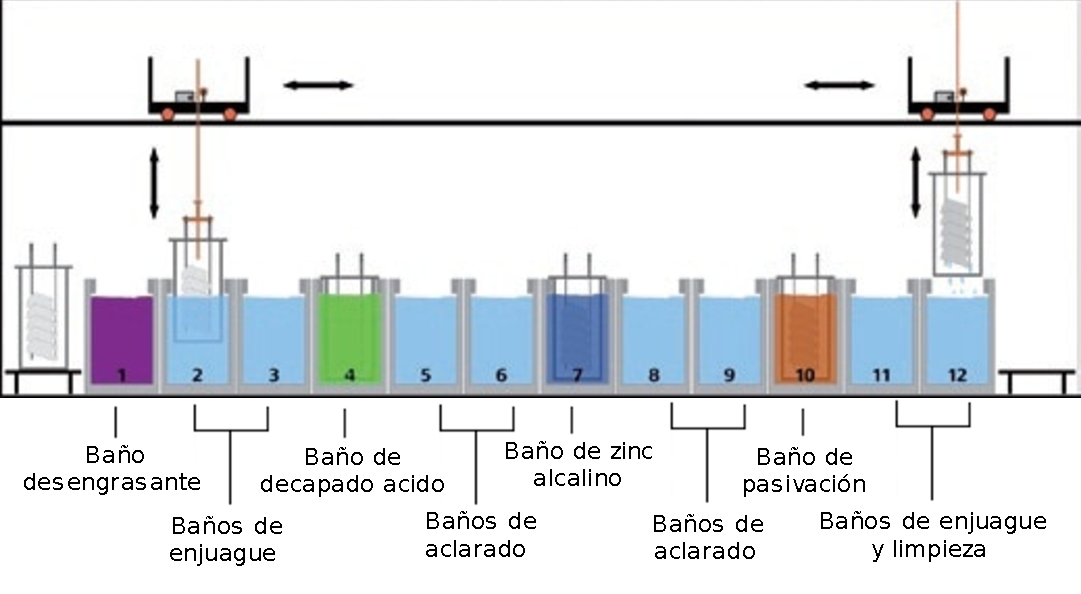
\includegraphics[width=1.0\textwidth]{Figures/Cap_2/diagrama_galvanizado_electrolitico}
	\caption{Proceso de galvanizado electrolítico a través de la inmersión del objeto en distintos baños químicos.}
	\label{fig:galvanizado_electrolitico}
\end{figure}

La forma utilizada en las placa de circuito impreso (PCB) es a través de la electrólisis del objeto dentro de una solución con sales metálicas, con una fuente de muy alta corriente continua de bajo voltaje, mas bloques del metal necesario para el galvanizado. En la figura \ref{fig:copper_electroplating} se muestra un caso donde el ánodo es de cobre y el cátodo es el PCB a galvanizar. 

\begin{figure}[h]
	\centering
	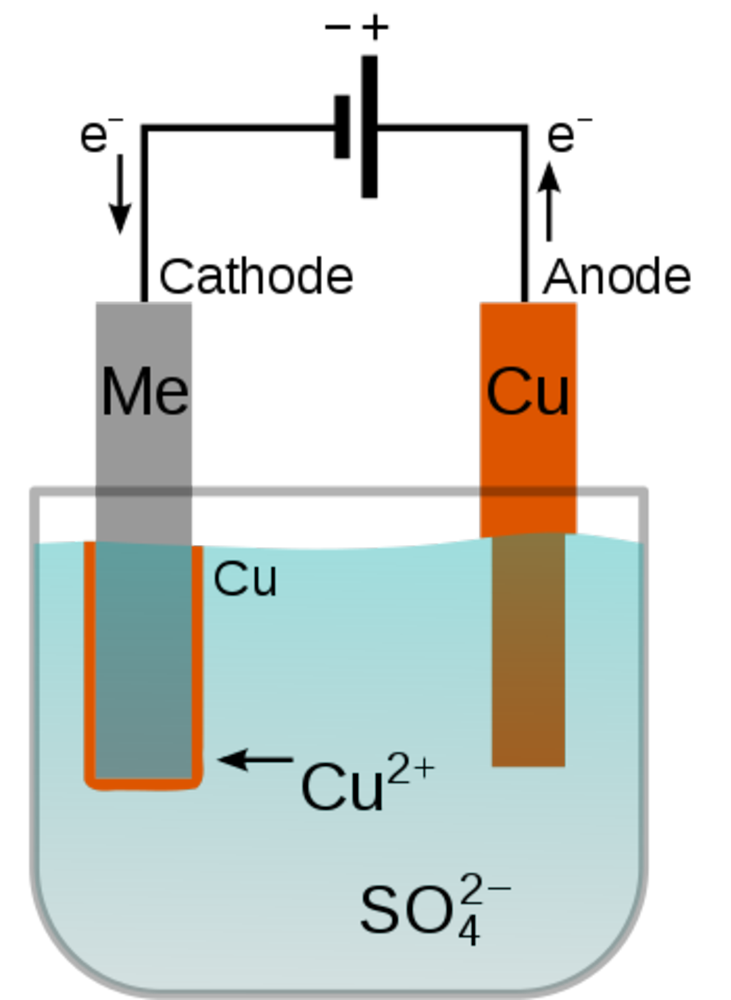
\includegraphics[width=0.3\textwidth]{Figures/Cap_2/galvanizado_copper_electroplating}
	\caption{Proceso electrolítico a través del cual se fija la capa de material sobre la superficie del objeto.}
	\label{fig:copper_electroplating}
\end{figure}


\subsection{ Proceso de galvanizado por electrólisis }

En la fabricación de PCBs se parte de un material base de sustrato de laminas epoxi FR4 revestido con laminas de cobre. Este debe ser sometido previo a realizar la electrólisis en sí, a una sucesión de baños químicos para limpiar y homogeneizar toda las partes metálicas de superficie. El proceso es repetido con variantes del metal galvánico para lograr el circuito final. 

En el proceso de fabricación de un PCB se utilizan aproximadamente 10 etapas distintas entre dos procesos. El primer proceso incluye el galvanizado con cobre de las vías entre capas, sobre el material laminado previamente perforado. El segundo proceso incluye el grabado del circuito impreso en si, previamente fijada la imagen negativa sobre las superficies del mismo.
Existe una similitud en muchos de los pasos de inmersión de las placas en los productos químicos, que resulta en controlar mismos parámetros en las distintas cubas a lo largo del proceso. 
En la Figura \ref{fig:diagrama_proceso} se muestra los efectos producidos sobre un perfil de una vía en un sustrato FR4, para las etapas mas relevantes.

\begin{figure}[h]
	\centering
	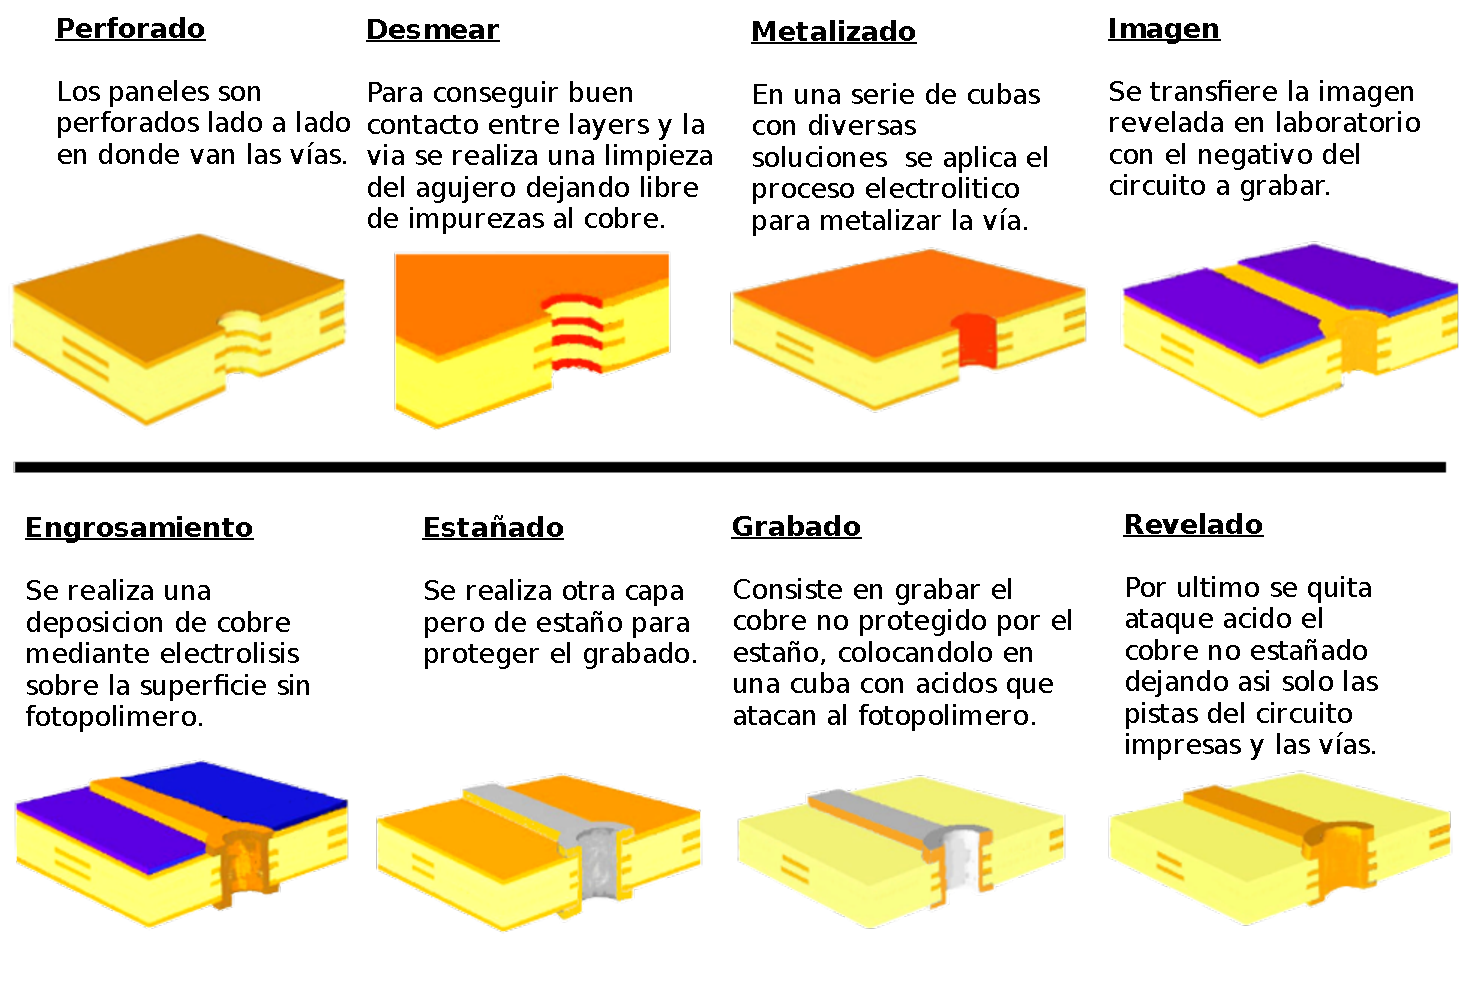
\includegraphics[width=1.0\textwidth]{Figures/Cap_2/diagrama_galvanizado_completo}
	\caption{ Diagrama simplificado de las etapas \footnotemark. \footnotemark.}
	\label{fig:diagrama_proceso}
\end{figure}

\footnotetext{\url{https://www.4pcb.com/media/presentation-how-to-build-pcb.pdf}} 
\footnotetext{SASE2013-Circuitos Impresos de Marcos Mayer} 

En el proceso desarrollado en Daichi S.A. la serie completa, desde que se cortan los paneles FR4 hasta que se coloca la mascara antisoldante, incluye entre 20 a 25 de pasos los cuales se resumen a continuación lo mas importantes.
% Agregar una TABLA con los pasos segun etapa a grandes rasgos.
% *************************************************************************

La figura \ref{fig:galvanizado_pcb} muestra el resultado final de un PTH (Plated Through Hole o agujero pasante metalizado) o  vía, de un un PCB.
\begin{figure}[h]
	\centering
	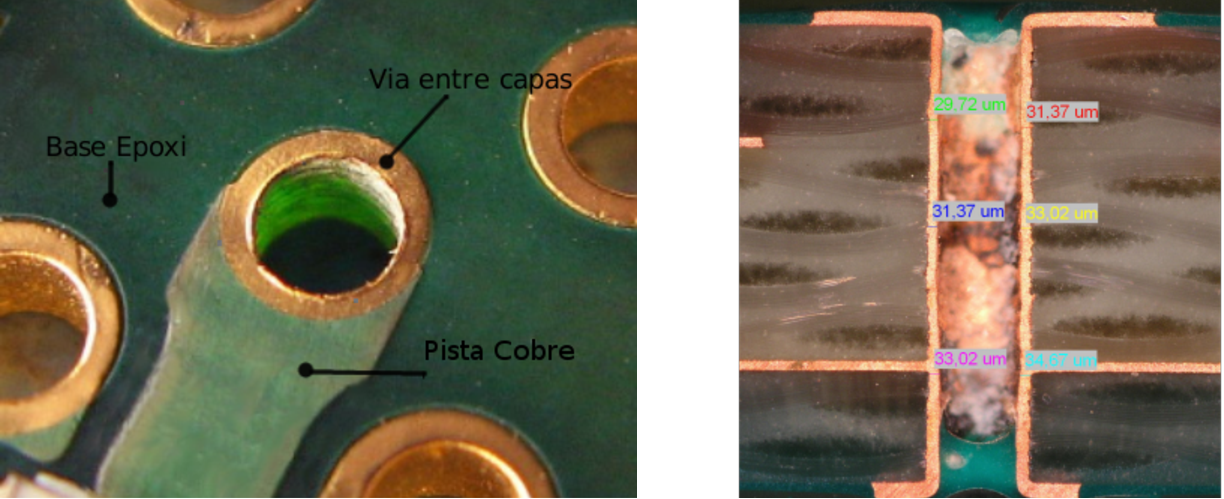
\includegraphics[width=.8\textwidth]{Figures/Cap_2/galvanizado_pcb_2}
	\caption{Vía entre capas galvanizada en un PCB}
	\label{fig:galvanizado_pcb}
\end{figure}

\section{ Parámetros críticos del galvanizado }

En el proceso de galvanización de PCBs el control de ciertos parámetros físicos-químicos en cada una de las etapas es fundamental para garantizar la uniformidad y calidad del baño metálico. 

En las diferentes bateas de la linea de galvanizado es necesario controlar, según cada etapa uno o algunos de los siguientes parámetros físicos-químicos del proceso:
\begin{itemize}
	\item Temperatura.
	\item Nivel de líquidos.
	\item Conductividad o concentración de iones.
	\item Corriente entregada (electrólisis).
	\item Inyección de aire.
\end{itemize}

Actualmente en la linea de galvanizado los operadores cuentan solo con su experiencia y con el soporte de instrumental de medición básico que poseen en algunas las etapas de la linea. Para saber cuando una etapa esta finalizada se basan en el tiempo que saben funciona y por observación del estado del proceso. Esto puede acarrear muchos problemas si no se han estandarizado procesos. Además es causante de que el producto final muchas veces no tenga una calidad estándar y de que no se puedan prevenir fallas del proceso a tiempo.
 
Por todo esto para saber cuando un proceso fue realizado correctamente, es necesario tener información precisa, detallada y respetar los tiempos e indicadores preestablecidos para lograr el tipo de galvanizado buscado. 

\subsection{ Fallas en el galvanizado de PCBs }

En la producción de PCBs el resultado final correcto es aquel en donde el espesor del baño metálico es uniforme en toda la superficies y paredes de las vías. Cuando este proceso no ocurre correctamente se originan distintas fallas, de las cuales las más comunes son:
\begin{itemize}
	\item Vías sin galvanizar.
	\item vías obstruidas por exceso de cobre.
	\item Laminado no uniforme de metal cobre.
	\item Micro cortes del cobre y puntos de no conductividad.
\end{itemize}

En la figura \ref{fig:thr_incorrecto_perfil} se observan las distintos grosores de cobre con vías mal galvanizadas en función de su ubicación en el sustrato del PCB y la cercanía al ánodo de cobre.

\begin{figure}[h]
	\centering
	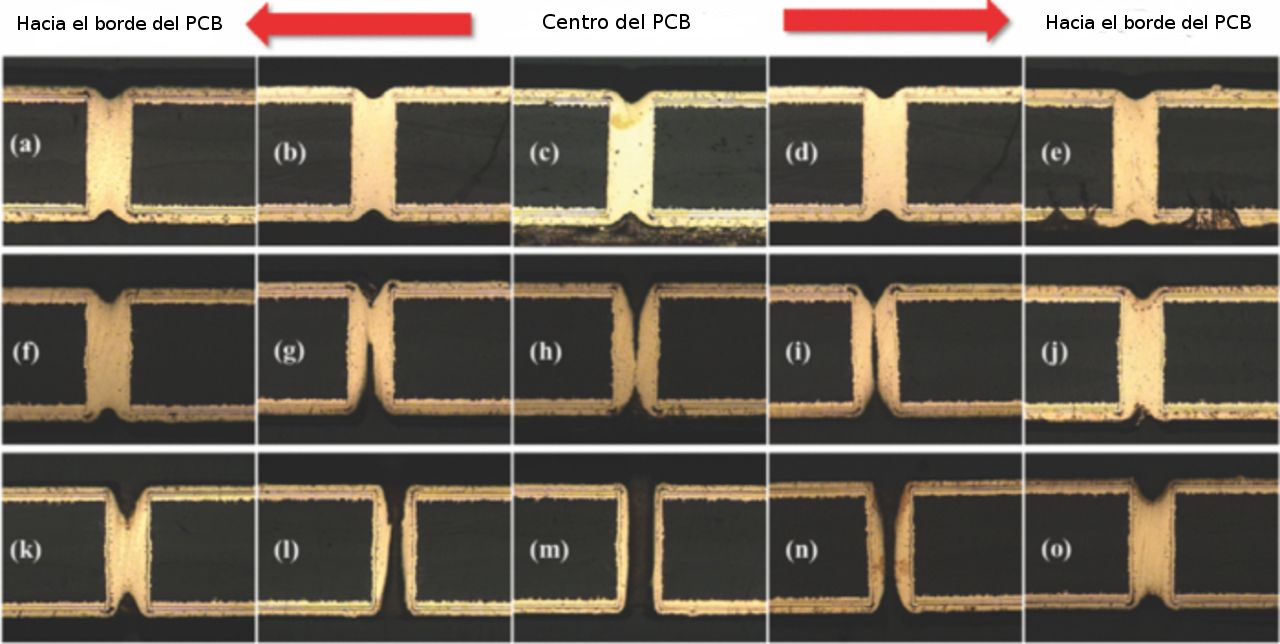
\includegraphics[width=.9\textwidth]{Figures/Cap_2/through_hole_perfil_fallado}
	\caption{Perfil de vías según la ubicación relativa en los sustratos y el los cátodos.}
	\label{fig:thr_incorrecto_perfil}
\end{figure}

En la figura \ref{fig:fallas_en_PTH} se observa los problemas originados por la mala preparación previa de las superficies metálicas del sustrato, originado puntos sin continuidad o circuitos abiertos que lo volverán no aptos para la producción de circuitos.

\begin{figure}[h]
	\centering
	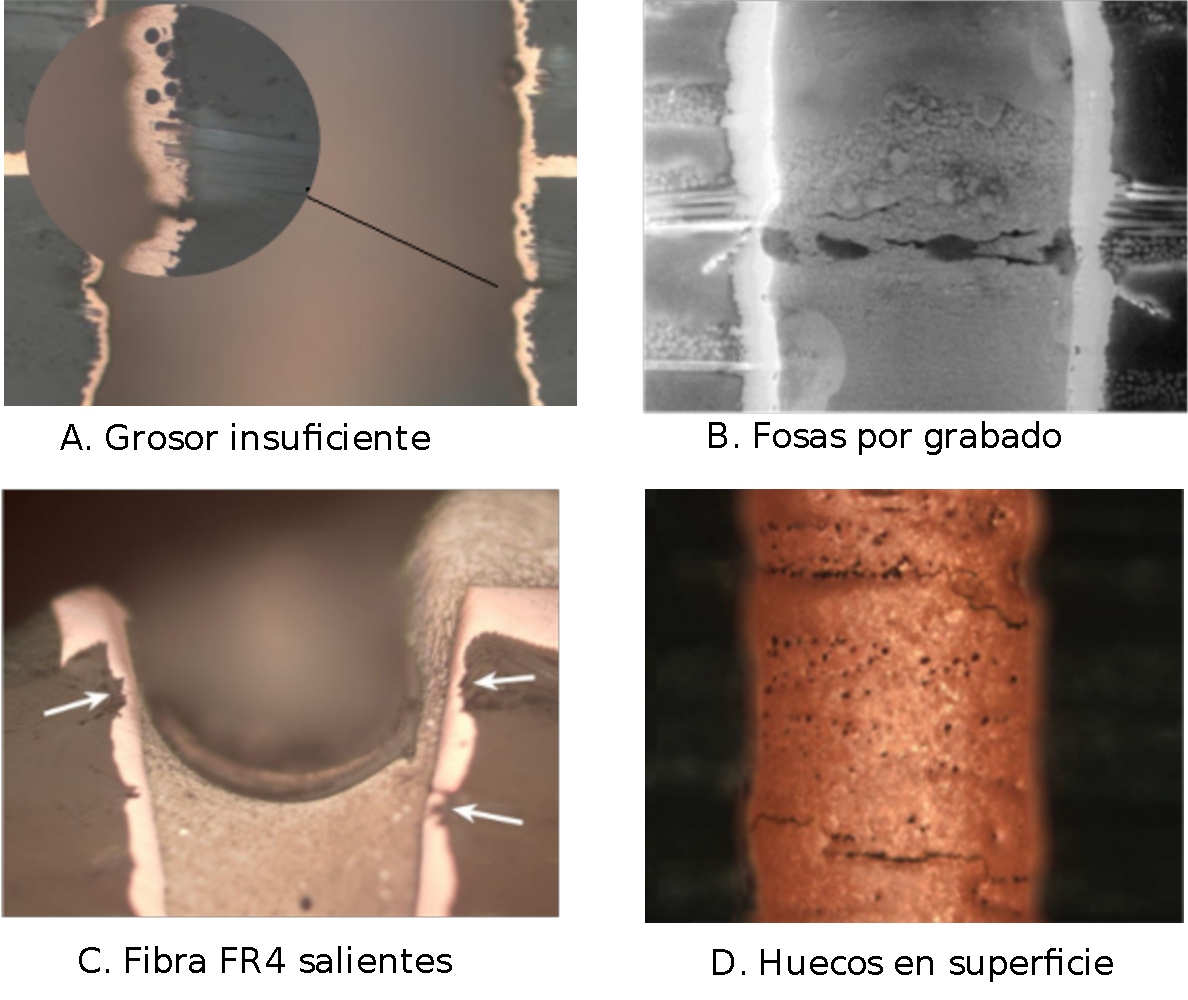
\includegraphics[width=.8\textwidth]{Figures/Cap_2/fallas_en_PTH}
	\caption{ Las capas de cobre se alejan del borde del orificio.}
	\label{fig:fallas_en_PTH}
\end{figure}

\section{ Determinación de la solución a utilizar } 

A fin de lograr recopilar los detalles de la arquitectura del sistema desarrollado, es necesario primero definir y determinar casos de uso, requerimientos técnicos y definiciones generales originados por la nueva planta, su operación y las necesidades del cliente. 

\subsection{ Definiciones Generales }

La linea cuenta con varias etapas en forma consecutiva independientes entre si pero con parámetros característicos similares, se determinó implementar un solo prototipo capaz de procesar el conjunto de parámetros del proceso, capaz de interactuar con los distintos usuarios del entorno y configurable según las etapas a monitorear.

El sistema debe funcionar entonces en modo predeterminado según los distintos escenarios posibles dentro de las etapas del proceso. De esta manera con un mismo hardware mas los sensores y actuadores necesarios, se puede supervisar y controlar las partes del proceso que se crean necesarias. En la figura \ref{fig:banco_pruebas} se muestra la implementación del banco de prueba que se diseño para la validación del prototipo.

\begin{figure}[h!]
	\centering
	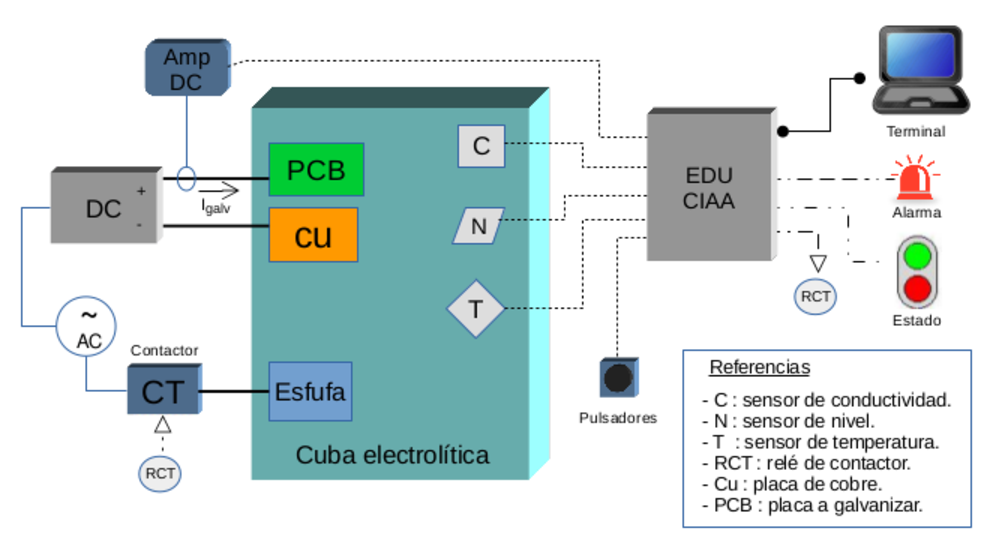
\includegraphics[width=1.2\textwidth]{Figures/Cap_2/diagrama_prototipo}
	\caption{Banco de pruebas de validación del prototipo. }
	\label{fig:banco_pruebas}
\end{figure}

En una etapa posterior luego de la validación del prototipo el cliente desarrollará un hardware a medida para usar en su planta. El mismo será producido en las cantidades necesarias según el numero de etapas que se determinen. Por ultimo estos distintos módulos funcionarán de manera independiente entre si.

% AGREGAR UNA IMAGEN DEL PROTOTIPO QUE SE PENSABA CONSTRUIR Y COMO SE PROBARIA A MODO DE BOSQUEJO.


\subsection{ Casos de Uso }
\label{subsec:casos_de_uso}
Los casos de uso del sistema se definen para determinar como se vincula éste con los distintos usuario, en función del modo de funcionamiento posible. Estos quedan entonces predeterminados por los escenarios posibles que se pueden originar en la operación de la linea. Los casos mas relevantes son:

\begin{enumerate}
	\item Puesta en alta y configuración del dispositivo, usado por personal técnico.
	\item Puesta en marcha en modo de funcionamiento 1, usado por el operario y el técnico.
	\item Puesta en marcha en modo de funcionamiento 2, usado por el operario y el técnico.
\end{enumerate}

Los modos 1 y 2 se refieren a dos configuraciones a partir de los escenarios mas comunes de conexión del prototipo. A fin de simplificar la puesta en marcha en campo y por la limitación de numero de entradas analógicas de la EDU-CIAA.
En la tabla \ref{modos_funcionamiento} se observa un resumen de los periféricos involucrados en cada caso.

%TABLA ****************
\begin{table}[h!]
\begin{flushleft}
\begin{tabular}{|m{1,2cm}|m{4cm}|m{4cm}|m{4cm}|} \hline
{\textbf{Modo}} & {\textbf{Función}} & {\textbf{Entradas}} & {\textbf{Salidas}}\\ \hline
{\textit{Func 1}} & {Controla nivel, temperatura, conductividad del liquido en la cuba.} & { Nivel tanque, temperatura del liquido, conductividad del liquido.} & {Contactor calefactor, contactor válvula de recambio, alarma de estado.} \\ \hline
{\textit{Func 2}} & {Controla nivel, temperatura, energía consumida en la cuba.} & {Nivel tanque, temperatura del liquido, corriente entrante.} & {Contactor calefactor, contactor válvula de recambio, alarma de estado.} \\ \hline
{\textit{Config.}} & {Modifica pines asignados, valores de alarma, tiempos de muestreo.} & {Comandos por terminal de pc.} & {Confirmación por terminal de pc y leds.} \\ \hline
\end{tabular}
\end{flushleft}
\caption{Descripción modos de funcionamiento.}
\label{modos_funcionamiento}
\end{table}

En la Figuras \ref{fig:casoUsoAlta} y \ref{fig:casodeUso1y2} se notan las interacciones entre los distintos submódulos del sistema en función de los casos de usos y los usuarios vinculados.

\begin{figure}[h!]
	\centering
	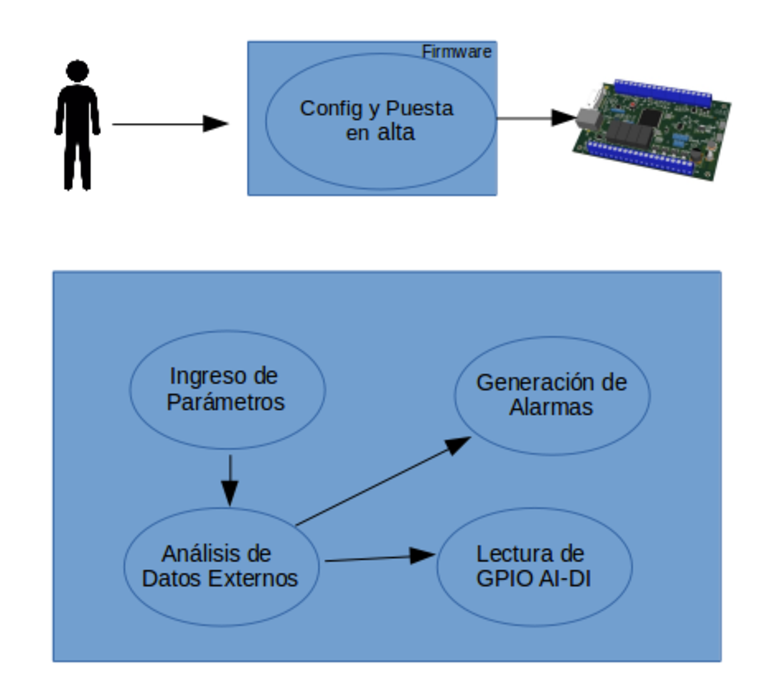
\includegraphics[width=.9\textwidth]{Figures/Cap_2/caso_uso_Alta_UML}
	\caption{Diagrama UML caso de uso de puesta en alta.}
	\label{fig:casoUsoAlta}
\end{figure}

La puesta en alta es el momento en que se determinan a través de la interfase terminal HMI (Humman Machine Interface o interfase hombre maquina) las parámetros a medir y configuraciones de los puertos del hardware.

\begin{figure}[h!]
	\centering
	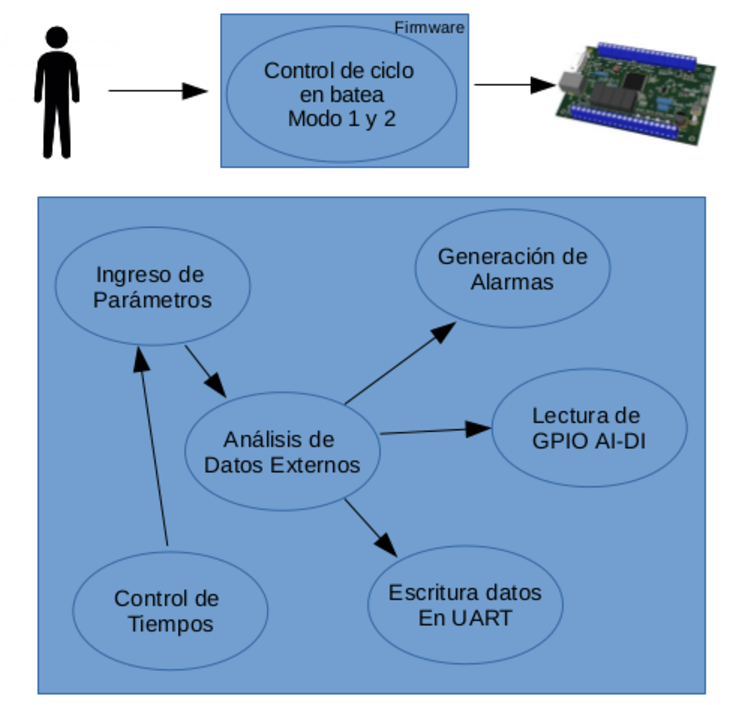
\includegraphics[width=.8\textwidth]{Figures/Cap_2/caso_uso_Marcha_UML}
	\caption{Diagrama UML de casos de uso Modo 1 y 2.}
	\label{fig:casodeUso1y2}
\end{figure}

En el Apéndice \ref{AppendixA} se detallan la secuencias involucradas en cada una de los casos de uso.

\subsection{ Requerimientos funcionales y no funcionales }
\label{subsec:Requerimientos}

A continuación se enumera lista completa con los requerimientos surgidos del análisis en conjunto con el personal de la planta tanto del problema, los casos uso y las prestaciones que tendrá la nueva planta. 
Cabe mencionar que la lista de requerimientos se originó previamente en la materia \emph{Gestión de Proyectos} del posgrado.

\begin{enumerate}
%------------------------------------------------------------------------
\item Requerimientos Funcionales
\begin{enumerate}

\item Temperatura (RFTEM)
\begin{enumerate}
\item El sistema medirá la temperatura con un resolución de XX, cada YY segundos.
\item El sistema mantendrá la temperatura controlada según los parámetros configurados por el usuario.
\item El sistema elevará la temperatura a través de la activación de una salida digital conectada a una resistencia.
\item La activación de la resistencia se implementará a través de una ventana Smith Trigger para evitar la intermitencia y generación de ruido en las líneas de alimentación principal. Cruce por 0.
\item En caso de que la temperatura se exceda de rango de considerar interrumpir el proceso y emitir una alarma.
\item El sistema almacenará al menos XX valores de temperatura en un archivo en memoria flash.
\end{enumerate}

\item Energía (RFENE)
\begin{enumerate}
\item El software medirá la corriente total (DC) entregada al proceso de electrólisis cada XX segundos, con YY de resolución.
\item El software medirá la tensión aplicada (DC) entre los bornes del electrólisis cada XX segundos con YY de resolución.
\item El sistema almacenará al menos XX valores de corriente y tensión en un archivo en memoria flash.
\item Los rangos de valores óptimos de tensión y corriente serán tomados de los parámetros de lote ingresados por el usuario y mostrados por pantalla para su configuración manual en la fuente de alimentación principal.
\end{enumerate}

\item Conductividad (RFCOND)
\begin{enumerate}
\item El software calculará a través de la corriente y tensión medidas en el tanque de galvanización, la conductividad de la solución salina cada XX segundos con YY de resolución.
\item El software deberá compensar las eventuales desviaciones de la conductividad óptima a través de la activación de XX válvulas de aditivos.
\end{enumerate}

\item Interfaces Hombre-Máquina (RFHMI)
\begin{enumerate}
\item El sistema contará con una pantalla estado del sistema con variables a definir.
\item El sistema contará con un método de ingreso de parámetros de lote a procesar.
\item Deberá permitir ingresar parámetros en modo manual y otros en modo codificado.
\item Deberá brindar a través de una interfaz Ethernet los históricos almacenados en memoria flash de variables del proceso que necesiten ser auditadas tras una etapa o tras el proceso completo. El máximo de registros será de XX número de puntos en formato YY.
\end{enumerate}

\item Tiempos (RFTI)
\begin{enumerate}
\item El software llevará un conteo del tiempo entre cada baño en las bateas, desde el momento que se inicia hasta el final del proceso.
\item En cada etapa deberá avisar y esperar a que un operario habilite la iniciación de la siguiente etapa.
\end{enumerate}

\item Niveles de bateas (RFNB)	
\begin{enumerate}
\item Evaluará que los niveles dentro del galvanizador estén dentro de los rangos permitidos de operación.
\item En caso de algún nivel crítico se emitirán alarmas y se considera la interrupción del proceso.
\end{enumerate}

\end{enumerate}

%------------------------------------------------------------------------
\item Requerimientos de Interfaz
\begin{enumerate}

\item Temperatura (RITEM)
\begin{enumerate}
\item La temperatura será medida a través de un sensor analógico de tolerancia XX.
\item La temperatura se medirá en los tanques XX, lo que arroja un total de YY numero de entradas analógicas independientes.(+xxAI)
\end{enumerate}

\item Energía (RIENE)
\begin{enumerate}
\item Tendrá un sensor de alta corriente del tipo XX conectado en una entrada analógica, para la corriente de galvanizador. (+1AI)
\item Tendrá un sensor de tensión de tipo XX conectados a los bornes de galvanizador. (+1AI)
\end{enumerate}

\item Conductividad (RICOND)
\begin{enumerate}
\item Tendrá XX dispositivos dosificador/es conectados a salidas digitales. (+xxDO)
\end{enumerate}

\item Interfaces Hombre-Máquina (RIHMI)
\begin{enumerate}
\item Debe mostrar información a través de un puerto VGA/HDMI con una taza de refresco menor a XX segundos. (+1USB)
\item Tomará de una entrada serie USB los valores de lote. (+1USB)
\item Accionara a través de una salida digital una alarma sonora/lumínica en caso de algún tipo de falla. (+1DO, +1AO) 
\item Contará con uno o dos pulsadores a fin de poder detener y accionar el procesos de galvanización, conectados a una/dos entradas binarias.(+1/2DO)
\item Dispondrá de una conexión remota a través de Ethernet. (+1ETH)
\end{enumerate}

\item Niveles de bateas (RINB)
\begin{enumerate}
\item Tendrá XX sensores de nivel conectados a entradas digitales. (+xxDI)
\end{enumerate}

\end{enumerate}

%------------------------------------------------------------------------
\item Requerimientos no Funcionales (RNF)
\begin{enumerate}
\item Deberá ser probada la funcionalidad a través de un banco de pruebas que se ajuste al comportamiento del sistema. 
\end{enumerate}
%------------------------------------------------------------------------
\item Restricciones de Diseño (RD)
\begin{enumerate}
\item De los requerimientos de interfaz se resume que como mínimo el hardware deberá contar con las siguientes interfaces:\\
- Entradas analógicas (AI) >= 3	\\
- Entradas digitales (DI) >= 3	\\
- Salidas analógicas (AO) >= 1	\\
- Salidas digitales (DO) >= xx	\\
- Puerto USB (USB) = 2	\\
- Puerto RED (ETH) = 1	\\
\end{enumerate}
%------------------------------------------------------------------------
\item Requerimientos a Futuro (RAF)
\begin{enumerate}
\item Brindar información acerca de si es necesario realizar una limpieza de sistema. Se puede utilizar como parámetro el número de procesos que se ejecutaron 	 	 	
\item Deberá permitir loguearse antes de iniciar el proceso, así tener un responsable de operación.
\item Deberá interactuar con una cinta de transportación automática que llevará las placas de una batea a otra. Accionara los motores (paso a paso?) de transporte y de elevación.
\item Si no se respetan los tiempos el sistema deberá dejar asentado el técnico y las acciones manuales ejecutadas a fin de tener un histórico antes posibles fallas en el lote.
\end{enumerate}

\end{enumerate}

En función de estos se propuso implementar el proyecto sobre una plataforma EDU-CIAA \citep{CIAA} en conjunto con una placa de interfaz hecha a medida. 
Los parámetros definidos con XX son aquellos que no pudieron ser definidos en su momento con el cliente ¿?
Los RFHMI relacionados con el ingreso de lotes no pudieron implementarse en esta primer etapa del proyecto al no tener un sistema centralizado que controle las etapas.







